% !TeX spellcheck = en_US
\documentclass[letterpaper,12pt,twoside]{report}
\usepackage{fancyhdr}
\usepackage{fullpage}
\usepackage{tikz}
\usepackage{amsmath}

\begin{document}
	\pagestyle{fancy}
	\fancyhf{}
	\fancyhead[L]{Day 8}
	\fancyhead[R]{\textit{The Calendar Project}}
	\fancyfoot[L]{Citations Involved: none}
	
	% Problem
	\paragraph{Problem}
	\begin{quote}
	\textsf{This figure consists of four congruent rectangles with a common vertex and coincident sides as shown. The perimeter of each rectangle is $16$ cm. The perimeter of the shape is $48$ cm. Find the area of the shape.}
	\end{quote}
	
	% Graphics
	\begin{center}
		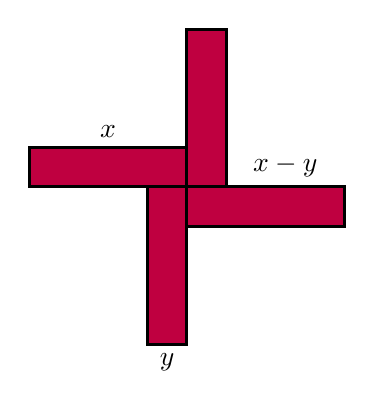
\begin{tikzpicture}[scale=0.5]
		\draw[very thick][fill=purple] (0,0) -- (-4,0) -- (-4,1) -- (0,1) -- cycle;
		\draw[very thick][fill=purple] (0,0) -- (0,4) -- (1,4) -- (1,0) -- cycle;
		\draw[very thick][fill=purple] (0,0) -- (-1,0) -- (-1,-4) -- (0,-4) -- cycle;
		\draw[very thick][fill=purple] (0,0) -- (0,-1) -- (4,-1) -- (4,0) -- cycle;
		
		\node[above] at (-2,1) {$x$};
		\node[below] at (-0.5,-4) {$y$};
		\node[above] at (2.5,0) {$x-y$};
		
		\end{tikzpicture}
	\end{center}
	
	% Reasoning
	\paragraph{Reasoning}
	\begin{quotation}
	
	Let the length of the rectangles be $x$ and their width be $y$. The figure above shows that each rectangle contributes $x+y+(x-y)=2x$ to the perimeter of the overall figure; with 4 such rectangles, this perimeter is $4(2x)=8x$. Given that this perimeter is $48\textrm{cm}$, $8x=48$ and therefore $x=6$.
	
	The rectangle perimeter formula is $2(x+y)$ in this situation (2); with $x=6$ plugged in and $16\textrm{cm}$ given as its value, $16=2(6+y)$, $8=6+y$, and $y=2$.
	
	The rectangle area formula is $xy$ in this situation (1); with $x=6$ and $y=2$ plugged in, the area of each rectangle is $(6)(2)=12\textrm{cm}^2$. With 4 such rectangles in the figure, its overall area is $4(12)=\boxed{48\textrm{cm}^2}$.
	
	\end{quotation}
	
	\paragraph{External References}
	
	\begin{enumerate}
		\item Textbook Ch. 9, Pg. 589: Area of Parallelograms
		\item Textbook Ch. 9, Pg. 590: \textit{Remember!}
	\end{enumerate}

\end{document}